\documentclass[12pt, a4paper]{article}
\usepackage[utf8]{inputenc}
\usepackage{amsmath,amsthm,amssymb}
\usepackage{mathtext}
\usepackage[T1,T2A]{fontenc}
\usepackage[english,russian]{babel}
\usepackage{url}
\usepackage{xurl}
\usepackage{listings}
\usepackage{titlesec}
\usepackage{xcolor}
\usepackage{booktabs}
\usepackage{hyperref}
\usepackage{float}
\usepackage{longtable}
\usepackage{array}
\usepackage{ragged2e}
\newcommand{\sectionbreak}{\clearpage}
\renewcommand{\thefigure}{\arabic{figure}}
\setcounter{secnumdepth}{0}
\setlength{\emergencystretch}{3em}

\hypersetup{pdfstartview=FitH, colorlinks=true, linkcolor=black, urlcolor=black}
\pagestyle{plain}
\usepackage{graphicx}
\usepackage[left=3cm,right=2cm,top=2cm,bottom=2cm,bindingoffset=0cm]{geometry}
\graphicspath{{img/}}

\newcolumntype{L}[1]{>{\RaggedRight\hspace{0pt}\arraybackslash}p{#1}}

\begin{document}
\begin{titlepage}
\newpage

\begin{center}
УНИВЕРСИТЕТ ИТМО
\end{center}

\vspace{4em}

\begin{center}
Факультет систем управления и робототехники \\
\end{center}

\vspace{6em}

\begin{center}
\large \textbf{Культура ИИ: Медиа и креативность\\
Итоговый проект\\
Последний пешеход: мультимедийная история}
\end{center}

\vspace{8em}

\newbox{\lbox}
\savebox{\lbox}{\hbox{Муравья Н.Р.}}
\newlength{\maxl}
\setlength{\maxl}{\wd\lbox}\addtolength{\maxl}{10pt}
\hfill\parbox{12cm}{
\hspace*{5cm}\hspace*{-5cm}Студент:\hfill\hbox to\maxl{
Маврин Г.А. \hfill}\\
\hspace*{5cm}\hspace*{-5cm}\hfill\hbox to\maxl{
группа R4175c \hfill}\\
\hspace*{5cm}\hspace*{-5cm}\hfill\hbox to\maxl{
ИСУ 368462 \hfill}\\
\\
\hspace*{5cm}\hspace*{-5cm}Преподаватель:\hfill\hbox to\maxl{\hfill Муравья Н.Р.}
}

\vspace{\fill}

\begin{center}
Санкт-Петербург \\2026
\end{center}

\end{titlepage}

\tableofcontents

% ============================================================
\section{Введение}

\subsection{Задача и выбранный вариант}
Итоговый проект курса требует создать цельную мультимедийную историю, произвести для неё медиа с помощью инструментов искусственного интеллекта и собрать работающий цифровой продукт. Из двух предложенных вариантов выбран второй --- мультимедийная история: он позволяет соединить сценарий, визуальную систему, звук и интерактивность в одном артефакте.

Продукт проекта --- интерактивный мини-сайт <<Последний пешеход>> (\emph{The Last Pedestrian}). Это история о памяти и идентичности: последний человек в засыпанном городе каждое утро находит на цельном снегу след, ведущий из ниоткуда в никуда, и идёт по нему, пока след не приводит к собственной двери. Зритель проходит шесть сцен, делает один выбор и получает один из двух финалов. Сессия занимает 3--5 минут, звук можно отключить.

\subsection{Стек и состав работы}
Сайт собран на Vite 5, React 18 и TypeScript 5.6, стили написаны на чистом CSS. Медиа генерировались через агрегатор нейросетей, музыку дал Stable Audio, шумы взяты из Freesound (CC0). Текст, сценарий и код создавались при участии большой языковой модели DeepSeek 4.1 Flash 1017 в режиме low reasoning. Отчёт оформлен в \LaTeX{} и повторяет шаблон лабораторных работ 5--7.

В работе есть паспорт истории, сценарий на 507 слов, шесть иллюстраций, три портрета, видео 12{,}79~с, музыка 39{,}4~с, два звуковых сигнала, собранный сайт, экономический расчёт, декларация использования ИИ и раздел о решениях и ограничениях.

\subsection{Критерий готовности}
Готовым результатом считается опубликованный статический сайт, в котором работают все шесть сцен, развилка и оба финала; медиа загружаются локально, без внешних CDN; на ширине 360~px ничего не разъезжается; при отключённом звуке история остаётся понятной; в отчёте приведены фактические затраты, честная декларация ИИ и обоснование ключевых решений.

% ============================================================
\section{Паспорт истории}

Паспорт фиксирует девять обязательных полей и задаёт рамку для всех дальнейших решений: жанра, визуального стиля, звука и интерфейса. Значения приведены в таблице~\ref{tab:passport}.

\begin{small}
\setlength{\tabcolsep}{3pt}
\begin{longtable}{@{}L{4cm}L{11.6cm}@{}}
\caption{Паспорт истории <<Последний пешеход>>}\label{tab:passport}\\
\toprule
\textbf{Поле} & \textbf{Значение} \\
\midrule
\endfirsthead
\toprule
\textbf{Поле} & \textbf{Значение} \\
\midrule
\endhead
\bottomrule
\endlastfoot
Название & <<Последний пешеход>> / \emph{The Last Pedestrian} \\
\addlinespace
Жанр & Холодный психологический детектив с элементами магического реализма; интерактивная новелла \\
\addlinespace
Целевая аудитория & Жюри и преподаватели ИТМО; зрители 18--35, любящие атмосферную интерактивную прозу и медленное кино. Сессия --- 3--5 минут, звук может быть выключен \\
\addlinespace
Логлайн & Последний, кто чистит улицы засыпанного города, каждое утро находит на цельном снегу следы, ведущие из ниоткуда в никуда, и красную перчатку. Идёт поиск <<последнего пешехода>>, пока не приходит понимание: следы собственные, а город каждое утро стирает память \\
\addlinespace
Тема & Память и идентичность. Поиск другого человека оказывается поиском себя. Снег --- забывание, след --- рассказ, перчатка --- единственное доказательство, что кто-то был здесь \\
\addlinespace
Место и время & Безымянный заснеженный город, третья неделя непрекращающейся метели. Время не указано намеренно. Одна улица, одна квартира, одна машина для уборки снега, одно радио \\
\addlinespace
Персонажи & \textbf{Миро} --- бесполый персонаж: пол не указан и не подразумевается; последний, кто чистит улицы, ненадёжный детектив, который ищет и забывает. \textbf{Голос радио} --- свидетель, повторяющий слова Миро, будто знал их первым. \textbf{Пёс} --- молчаливый спутник, единственный, кто <<помнит>>, но не может сказать \\
\addlinespace
Ключевые события & Город пуст; Миро ведёт дневник, и дневник переписывается; каждое утро --- свежий след от порога; Миро допрашивает радио, пса и запись самого себя; след приводит обратно к своей двери; предстоит решить, кем быть в этой истории \\
\addlinespace
Эмоция & Холодная тревога, переходящая в узнавание и тихое горе. Неразрешимое, скупое утешение; <<холодный эпос>> \\
\end{longtable}
\end{small}

Отдельно подчеркну: Миро --- бесполый герой. Пол не указан ни в сценарии, ни в промптах, ни в интерфейсе. Это не формальность, а содержательное решение: история о том, что человек не может удержать собственный образ, и гендерный признак здесь только навязал бы лишнюю определённость. В промптах поэтому стоит явное ограничение \texttt{androgynous, gender not readable}, а в широких кадрах фигура показана со спины или в капюшоне.

% ============================================================
\section{Идея и сценарий}

\subsection{Логлайн и тема}
Логлайн строится на детективной интриге, но разрешается не разоблачением, а узнаванием. Формально Миро ищет неизвестного пешехода; фактически ищет себя, потерявшего память. Снег в этой системе --- не погода, а городская служба забывания: он каждое утро содержит улицы в порядке, стирая следы. Перчатка --- единственный материальный предмет, который переживает стирание, поэтому именно она становится доказательством существования.

Сценарий написан в настоящем времени и без родовых окончаний, относящихся к Миро. Объём основного текста --- 507 слов: сцены 1--5 и оба финала, без заголовков, строк <<Ассеты>> и текстов интерфейса.

\subsection{Структура}
История состоит из пяти линейных сцен, одной развилки и двух финалов (таблица~\ref{tab:scenes}). Такая структура удерживает объём завершимым: зритель проходит короткий путь, но получает две разные тезы.

\begin{small}
\setlength{\tabcolsep}{3pt}
\begin{longtable}{@{}L{1.0cm}L{3.4cm}L{7.3cm}L{3.5cm}@{}}
\caption{Структура истории: сцены, содержание и взаимодействие}\label{tab:scenes}\\
\toprule
\textbf{№} & \textbf{Сцена} & \textbf{Что происходит} & \textbf{Действие зрителя} \\
\midrule
\endfirsthead
\toprule
\textbf{№} & \textbf{Сцена} & \textbf{Что происходит} & \textbf{Действие зрителя} \\
\midrule
\endhead
\bottomrule
\endlastfoot
1 & Утро. Свежий след & Пустая улица, след от порога в белую даль, Миро выходит с лопатой и записывает первую строку дневника & <<Дальше>> \\
\addlinespace
2 & Допрос радио & В кабине снегоуборщика радио повторяет слова Миро с одной изменённой фразой; выключить его не удаётся & <<Дальше>> \\
\addlinespace
3 & Дневник & Вчерашняя строка перечёркнута; Миро пытается вписать <<я>>, но грифель ломается; у края кадра появляется пёс & <<Дальше>> \\
\addlinespace
4 & След возвращается & Миро идёт по следу, улица делает круг и возвращает к той же двери; видео ведёт камеру вдоль следа & <<Дальше>> \\
\addlinespace
5 & Выбор & След упирается в порог; Миро не решается взяться за ручку & Выбор из двух вариантов \\
\addlinespace
6A & Финал A. <<Есть кто-то>> & Красная перчатка на своей руке; за спиной звучит второй, чужой шаг; радио называет имя Миро & Финал, повтор или другой выбор \\
\addlinespace
6B & Финал B. <<Снег ровный>> & Миро ложится в снег и почти сливается с полем; кадр белеет, звук уходит до одной ноты & Финал, повтор или другой выбор \\
\end{longtable}
\end{small}

\subsection{Развилка и два финала}
Развилка одна, и её формулировки задают не <<правильный>> и <<неправильный>> исход, а две разные тезы. Первая кнопка: <<Идти до конца --- значит, кто-то есть>>. Вторая: <<Стереть следы --- значит, остаться в одиночестве>>. Таймера нет, подсказки нет, оба пути равноправны.

Финал A подтверждает существование другого только звуком: шаг, имя, тёплая нота. Финал B отменяет поиск: Миро ложится в снег, и белое поле поглощает фигуру. Финальные строки зафиксированы заранее и не меняются: в финале A --- <<След был мой. Но шагов было два.>>, в финале B --- <<Снег ровный.>>.

\subsection{Твист}
Твист собран из повторов, а не из объяснения. Радио повторяет фразы Миро, дневник переписывает вчерашнюю запись, след замыкается на свою дверь, а в финале A Миро обнаруживает перчатку на собственной руке. Зритель получает улики в трёх модальностях --- текст, изображение, звук --- и собирает вывод сам. Объясняющего voice-over в сценарии нет: он убил бы двусмысленность и превратил историю в инструкцию.

\begin{figure}[H]
\centering
\begin{minipage}{0.48\textwidth}
\centering
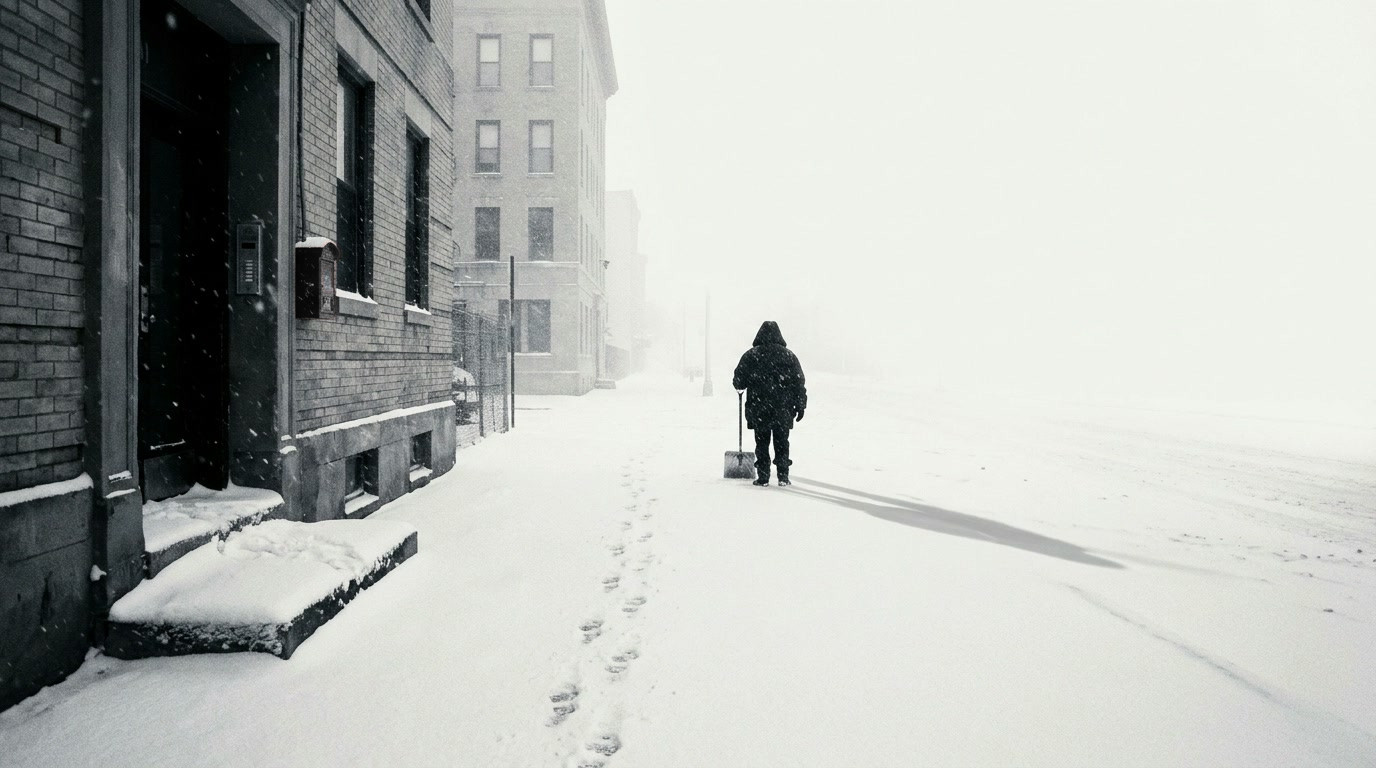
\includegraphics[width=\linewidth]{scene-1.jpg}
\end{minipage}
\hfill
\begin{minipage}{0.48\textwidth}
\centering
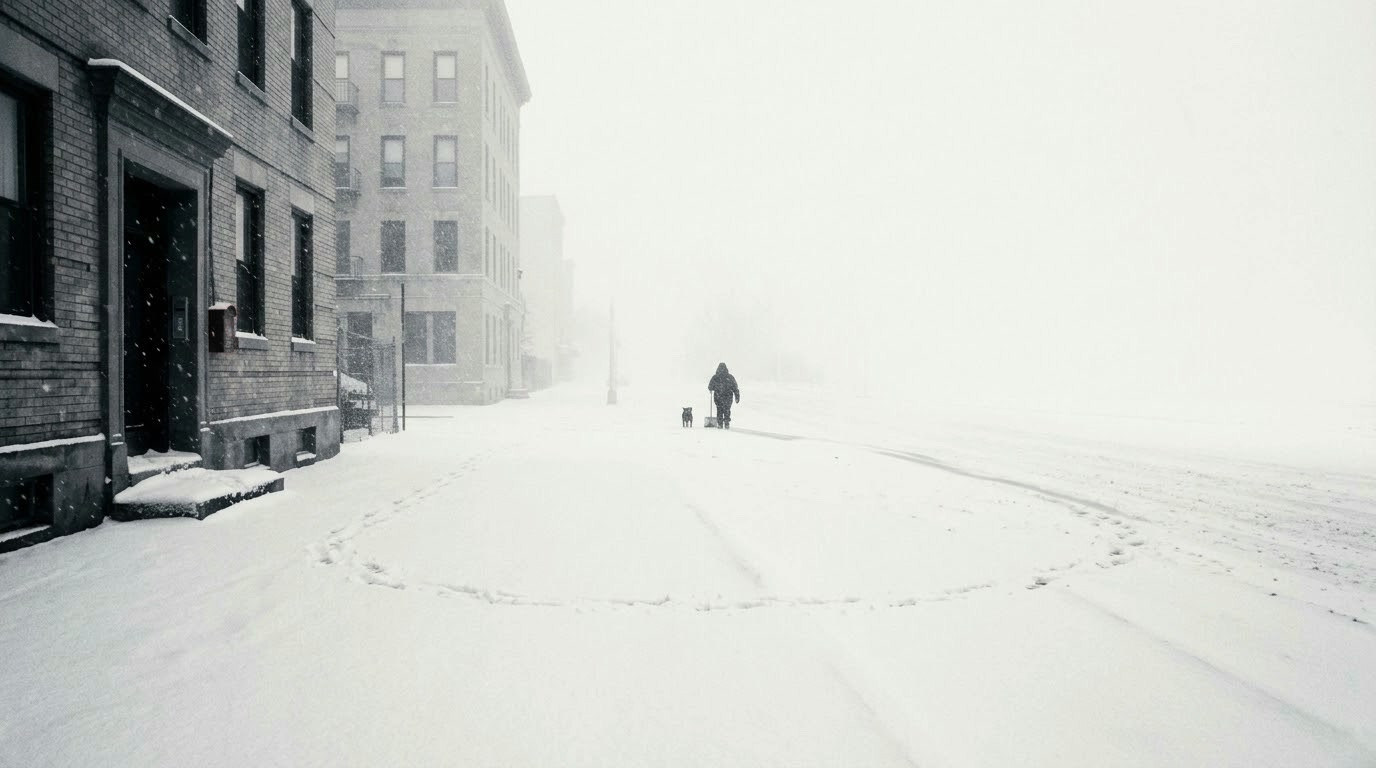
\includegraphics[width=\linewidth]{scene-4.jpg}
\end{minipage}
\caption{Завязка и петля: след начинается у порога (слева) и возвращается к той же двери (справа)}\label{fig:scenes}
\end{figure}

Композиция обоих кадров подчинена одной логике: 70--80\,\% площади занимает снег и воздух, фигура меньше 10\,\% высоты кадра, горизонт высокий или отсутствует. Зритель видит не героя, а пространство, в котором герой потерян.

% ============================================================
\section{Визуальная система и согласованность}

\subsection{Палитра, свет и композиция}
Визуальная система почти монохромна: четыре нейтральных тона и один красный акцент (таблица~\ref{tab:palette}). Красный существует ровно для одного объекта --- перчатки в финале A; во всех остальных кадрах его нет.

\begin{small}
\setlength{\tabcolsep}{4pt}
\begin{longtable}{@{}L{3.6cm}L{2.6cm}L{9.2cm}@{}}
\caption{Палитра иллюстраций}\label{tab:palette}\\
\toprule
\textbf{Токен} & \textbf{HEX} & \textbf{Назначение} \\
\midrule
\endfirsthead
\toprule
\textbf{Токен} & \textbf{HEX} & \textbf{Назначение} \\
\midrule
\endhead
\bottomrule
\endlastfoot
Снег & \texttt{\#F2F2EF} & Фон, снег, негативное пространство \\
\addlinespace
Чернила & \texttt{\#0B0C0D} & Текст, силуэты, глубокая тень \\
\addlinespace
Олово & \texttt{\#6E747A} & Средние тона, металл, вторичный текст \\
\addlinespace
Туман & \texttt{\#C9CDD0} & Воздушная дымка, границы, неактивные элементы \\
\addlinespace
Перчатка & \texttt{\#B3121C} & Единственный акцент: перчатка, один hover-штрих \\
\end{longtable}
\end{small}

Интерфейс сайта при этом использует тёмную тему (\texttt{--bg:\#0a0a0b}, текст \texttt{\#f4f6f8}, акцент \texttt{\#b4232a} --- близкий к палитре красного), поэтому визуальная система иллюстраций и оформление страницы не противоречат друг другу, а работают как две согласованные части одного продукта.

Свет всегда контровой: тёмная фигура на светлом поле, длинные тени, пересветы, чистые чёрные без провалов. Средние тона молочные и низкоконтрастные. Блум, блики и тёплый закат запрещены; допускается лишь лёгкое гало на ярких краях. Снег читается как плёночное зерно, а не как эффект частиц: он заполняет воздух, смягчает края и стирает расстояние. Композиция широкая и пустая; крупные планы разрешены только для дневника, руки и перчатки, но не для лица.

\subsection{Как обеспечивалась консистентность}
Шесть кадров, сгенерированных разными моделями, легко распадаются на шесть разных фильмов. Чтобы этого не произошло, применялась одна система приёмов.

\begin{enumerate}
\setlength{\itemsep}{2pt}
    \item \textbf{Единый style suffix.} В конец каждого промпта добавлялся один и тот же блок: палитра, контровой свет, зерно 35~мм, 70--80\,\% негативного пространства, фигура меньше 10\,\% высоты, запрет текста, лиц и тёплого света (листинг~1).
    \item \textbf{Style anchor.} Кадр \texttt{scene-1.jpg} сгенерирован первым и дальше прикладывался как reference image в image-to-image режимах; для сервисов без референса фиксировался один seed.
    \item \textbf{Силуэты вместо лиц.} Лицо невозможно удержать консистентным между генерациями, и оно навязывает эмоцию, которую история должна оставлять зрителю. Поэтому Миро --- спина, капюшон, рука; пёс --- силуэт сбоку; радио --- предмет.
    \item \textbf{Один красный объект на кадр.} Если генератор добавлял красное пятно, кадр либо отклонялся, либо проходил селективную десатурацию: все каналы, кроме красного, приглушались.
    \item \textbf{Отбор по чек-листу.} Каждый кадр проверялся на отсутствие текста, лиц, толпы, второго красного объекта, на совпадение света, горизонта и зерна с \texttt{scene-1.jpg}.
    \item \textbf{Постобработка.} Кроп до 1376$\times$768, JPEG q90, вес каждой сцены не более 205~КБ; лишний красный убирался точечно, а не глобальной десатурацией.
\end{enumerate}

\begin{figure}[H]
\centering
\begin{minipage}{0.48\textwidth}
\centering
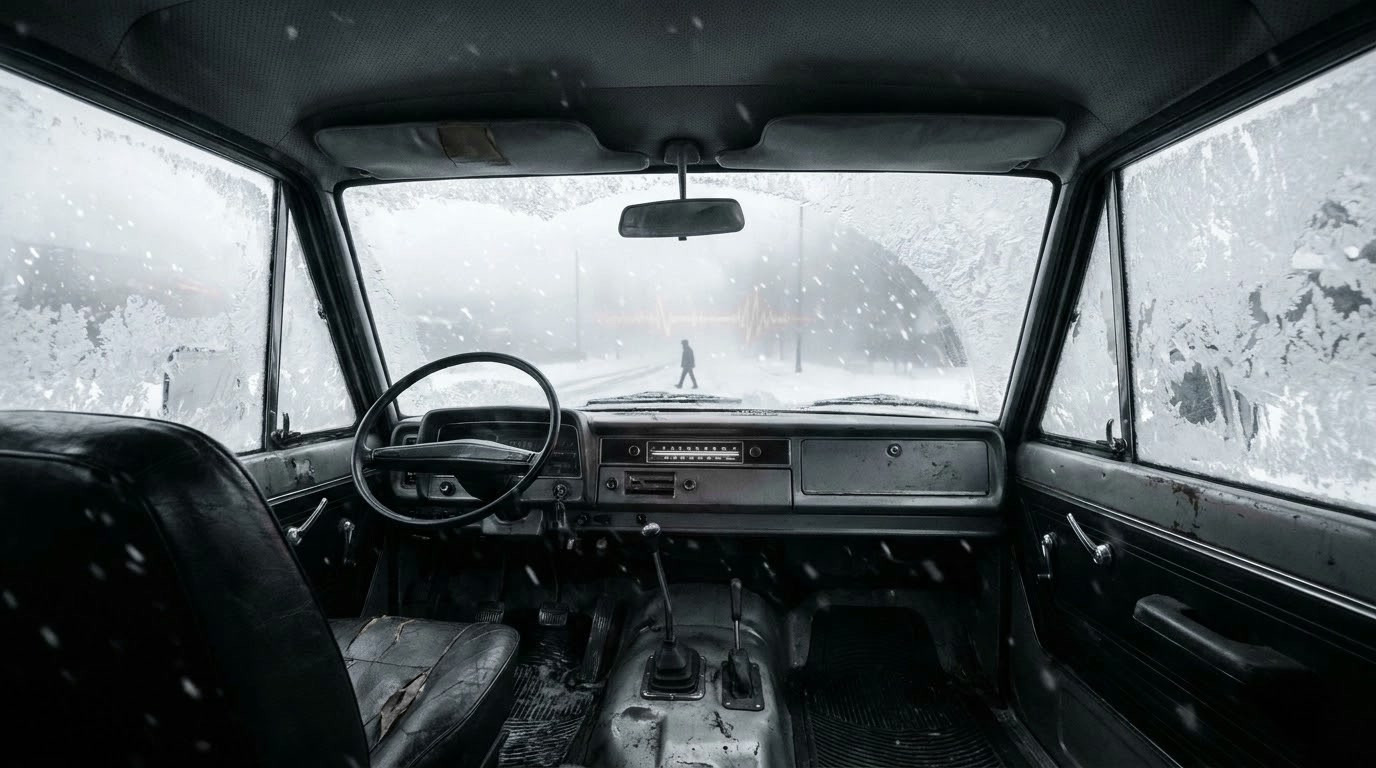
\includegraphics[width=\linewidth]{scene-2.jpg}
\end{minipage}
\hfill
\begin{minipage}{0.48\textwidth}
\centering
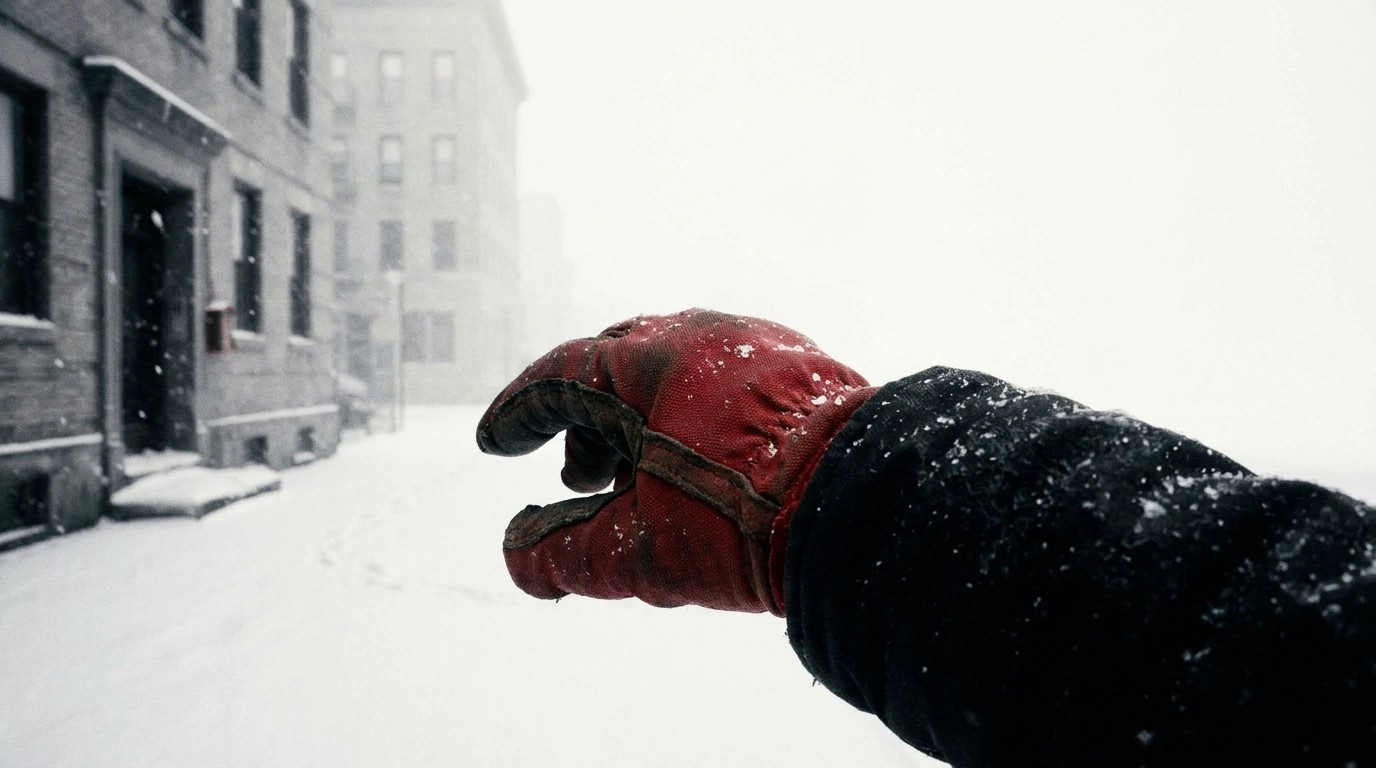
\includegraphics[width=\linewidth]{scene-5.jpg}
\end{minipage}
\caption{Интерьер кабины с единственным источником тепла (слева) и единственный кадр с красным акцентом (справа)}\label{fig:visual}
\end{figure}

На рис.~\ref{fig:visual} видно, как работает правило одного акцента: в кабине тёплой остаётся только шкала радио, но она не красная; в финальном кадре красной остаётся только перчатка, а всё остальное приведено к нейтральной шкале.

\begin{figure}[H]
\centering
\begin{minipage}{0.31\textwidth}
\centering
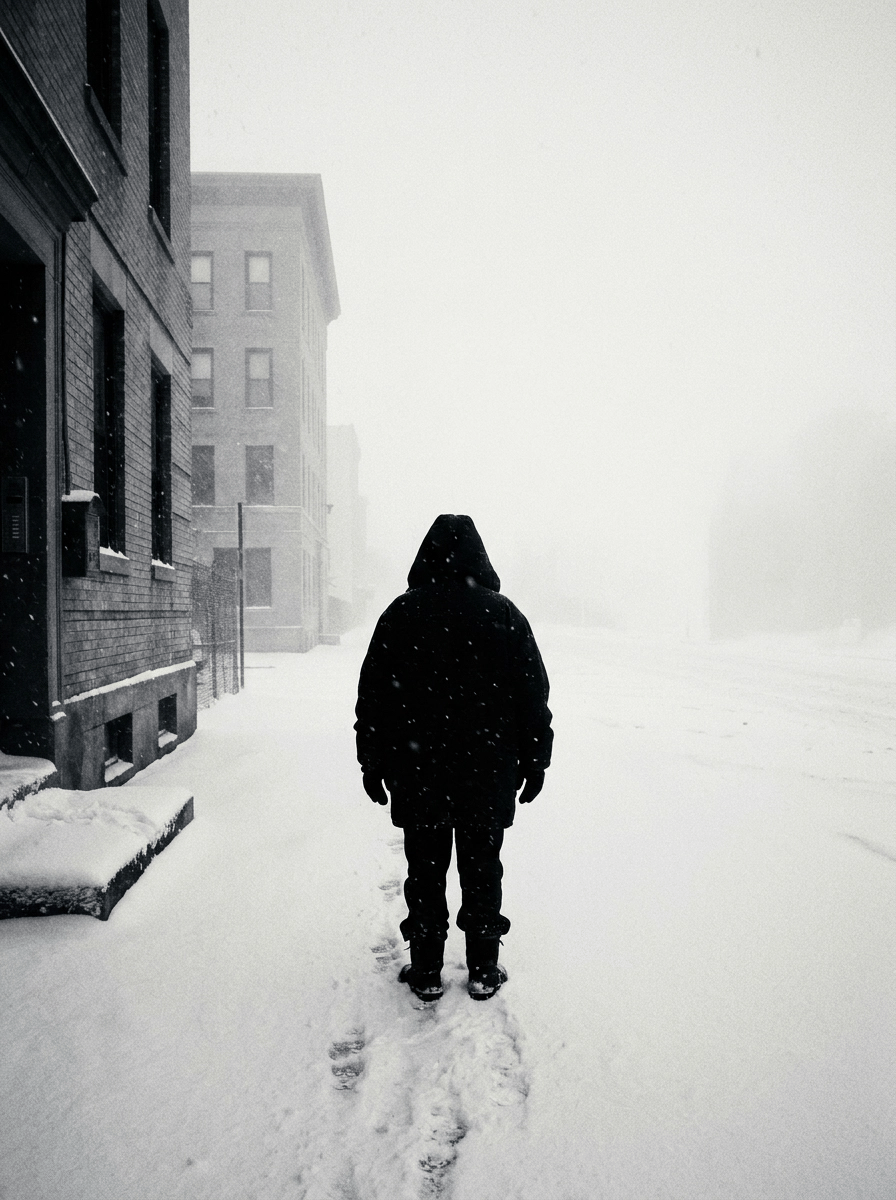
\includegraphics[width=\linewidth]{char-miro.png}
\end{minipage}
\hfill
\begin{minipage}{0.31\textwidth}
\centering
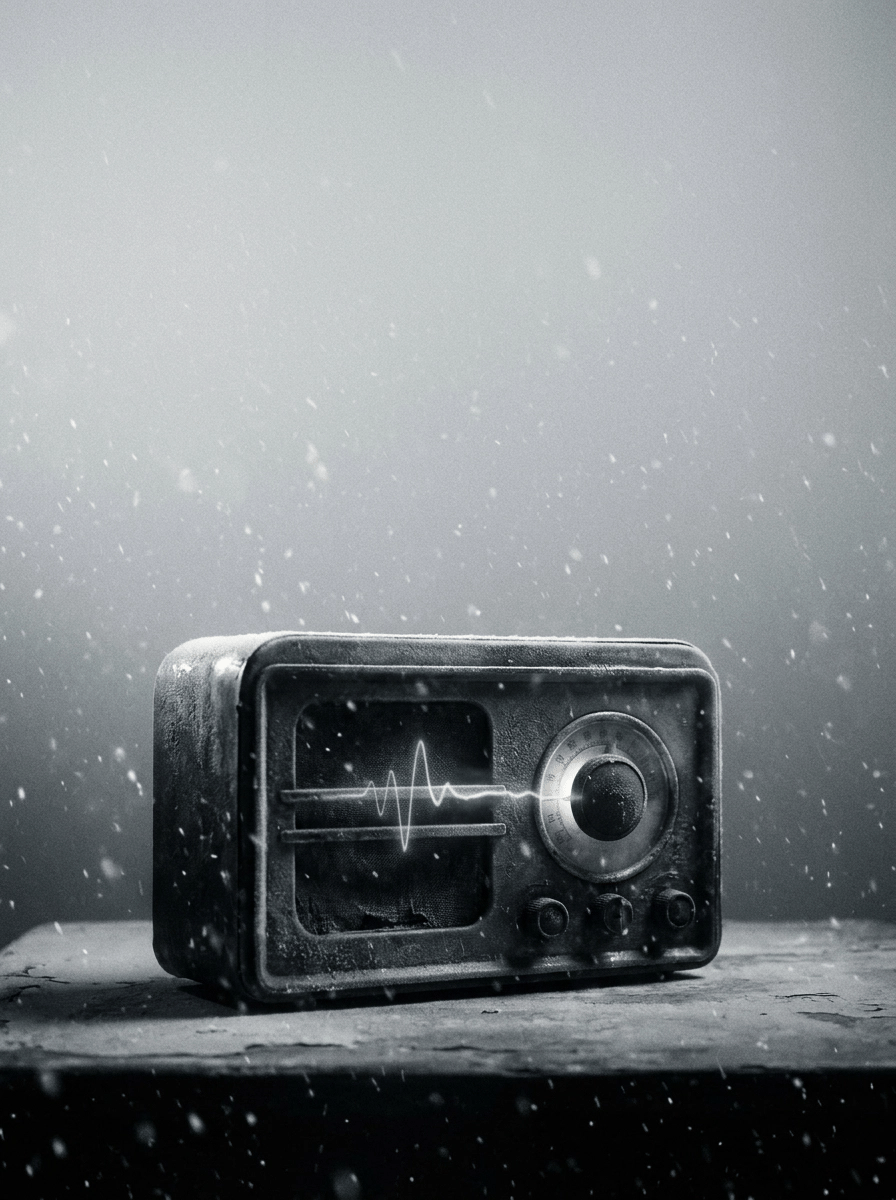
\includegraphics[width=\linewidth]{char-radio.png}
\end{minipage}
\hfill
\begin{minipage}{0.31\textwidth}
\centering
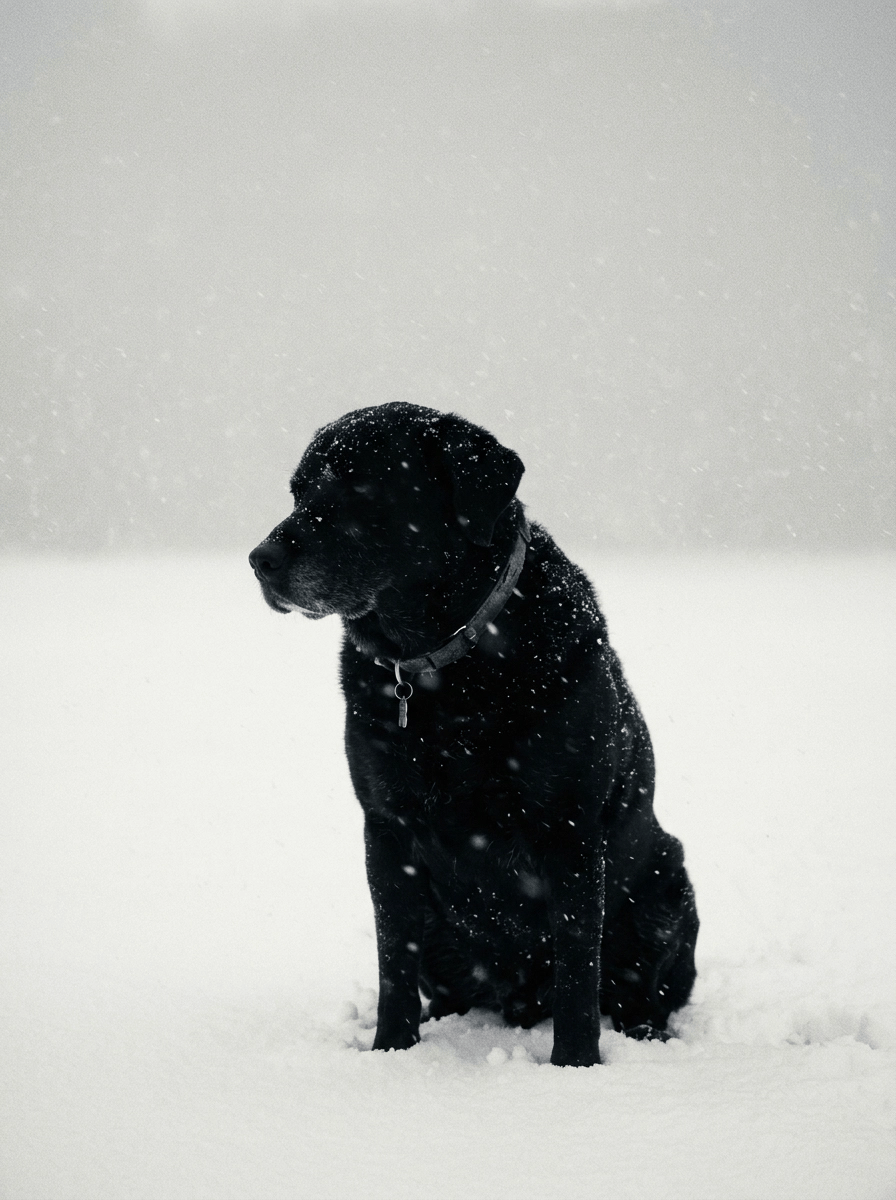
\includegraphics[width=\linewidth]{char-dog.png}
\end{minipage}
\caption{Карточки присутствия: Миро, Голос радио и Пёс. Портреты --- не character sheet, а силуэт, предмет и поза}\label{fig:portraits}
\end{figure}

Портреты (рис.~\ref{fig:portraits}) решены как <<карточки присутствия>>: единый туманно-серый фон, контровой свет, тонкая светлая кромка по контуру, формат 3:4. Миро показан в полный рост со спины, радио --- крупным планом как предмет, пёс --- по грудь. Ни в одном портрете нет читаемого лица и гендерных признаков.

% ============================================================
\section{Производство: сервисы и промпты}

\subsection{Сервисы и модели}
Все изображения, видео и синтетическая речь генерировались через агрегатор нейросетей с оплатой за генерацию; музыка --- в Stable Audio на бесплатном тарифе; шумы --- в Freesound, только CC0. Текст, сценарий, промпты и код создавались с помощью DeepSeek 4.1 Flash 1017 в режиме low reasoning. Фактический набор моделей и дат приведён в таблице~\ref{tab:services}.

\begin{small}
\setlength{\tabcolsep}{3pt}
\begin{longtable}{@{}L{4.0cm}L{5.0cm}L{2.0cm}L{4.0cm}@{}}
\caption{Сервисы, модели и даты производства}\label{tab:services}\\
\toprule
\textbf{Этап} & \textbf{Сервис / модель} & \textbf{Дата} & \textbf{Результат} \\
\midrule
\endfirsthead
\toprule
\textbf{Этап} & \textbf{Сервис / модель} & \textbf{Дата} & \textbf{Результат} \\
\midrule
\endhead
\bottomrule
\endlastfoot
Текст, сценарий, промпты, код & DeepSeek 4.1 Flash 1017, low reasoning & 13--14.11.2026 & \texttt{script.md}, \texttt{assets-prompts.md}, сайт \\
\addlinespace
Иллюстрации & Агрегатор: nano-banana-pro, nano-banana-2, nano-banana-2-1 & 13.11.2026 & 6 кадров \\
\addlinespace
Портреты & Агрегатор: nano-banana-pro, grom-art, nano-banana-2-1 & 13.11.2026 & 3 портрета \\
\addlinespace
Видео & Агрегатор: kling-v3-omni & 13.11.2026 & 12{,}79~с, без звука \\
\addlinespace
Музыка & Stable Audio, бесплатный тариф & 13.11.2026 & 39{,}4~с \\
\addlinespace
Голос радио & Агрегатор: tts-eleven-v4, tts-llm & 13.11.2026 & 4 генерации отклонены \\
\addlinespace
Шумы & Freesound, только CC0 & 13.11.2026 & \texttt{cue-step}, \texttt{cue-radio} \\
\end{longtable}
\end{small}

\subsection{Промпты}
Ниже приведены ключевые промпты дословно. Полный prompt bible с негативами и критериями отбора --- в исходном документе \texttt{docs/production/assets-prompts.md}.

\noindent\textbf{Листинг 1 --- иллюстрация \texttt{scene-1.jpg}, style anchor:}
{\scriptsize
\begin{verbatim}
Extreme wide shot of an empty snowbound city street at dawn, one lone
apartment doorway on the left, a single fresh line of footprints starting
at that doorstep and running straight into white distance, a tiny snowplow
operator in a heavy dark work coat with the hood up, androgynous, gender
not readable, standing with their back turned, shovel in hand, no other
people, near-monochrome palette of snow white #F2F2EF, ink black #0B0C0D,
tin gray #6E747A and fog gray #C9CDD0, with a single saturated red #B3121C
accent only where specified; contre-jour backlight, long shadows, blown
highlights, milky low-contrast midtones, clean blacks; heavy falling snow
as film texture; extreme wide composition, 70-80% negative space, tiny
human figure under 10% of frame height, centered or lower-third; shot on
35mm film, fine visible grain, subtle halation on bright edges; cold epic,
quiet, still; no text, no logos, no watermark, no crowd, no visible face,
no warm sunlight, no teal-orange grade, no lens flare, no bloom, 16:9
\end{verbatim}
}

\noindent\textbf{Листинг 2 --- видео \texttt{scene-4.mp4}, image-to-video:}
{\scriptsize
\begin{verbatim}
Slow low tracking shot moving forward along a single line of footprints in
deep snow, heavy snowfall drifting across the frame, a tiny figure in a
dark coat walking ahead with their back turned, hood up, androgynous,
gender not readable, a dark dog beside them, camera stays at knee height,
steady glide, no cuts, no camera shake, footprints gradually disappearing
under fresh snow behind the camera, near-monochrome snow white and ink
black and tin gray, 35mm film grain, cold epic, 12 seconds
\end{verbatim}
}

\noindent\textbf{Листинг 3 --- музыка \texttt{theme.mp3}:}
{\scriptsize
\begin{verbatim}
30-40 second loopable cold ambient score for an existential winter film,
low cello and contrabass drone, wide wind, distant metal creaks, faint
radio static, slow sub pulse entering midway, sparse prepared piano hit,
no melody lead, no vocals, no drums, no percussion, bleak, spacious,
cinematic, slow, seamless loop
\end{verbatim}
}

\subsection{Отбор и доработка}
Производство шло по принципу <<сначала дешёвый черновик, потом финал>>. На каждый ассет отводилось до трёх--пяти попыток; если пять подряд давали плохой результат, менялся сервис или упрощался кадр, а не переписывался промпт бесконечно. Все попытки, включая отклонённые, записывались в журнал генераций --- он же стал источником экономических цифр.

Итог: 13 генераций изображений на 9 принятых ассетов (6 иллюстраций и 3 портрета), одна генерация видео, одна генерация музыки, четыре генерации TTS и три генерации шумов. Почти все изображения приняты с первой или второй попытки.


\subsection{Отбраковка}
Три случая показывают, как отбор менял результат.

\begin{itemize}
\setlength{\itemsep}{2pt}
    \item \textbf{\texttt{scene-5.jpg}.} Первая версия была собрана композитом из двух генераций: на стыке читался прямоугольный шов и разница резкости. Кадр отклонён и перегенерирован целиком; затем выполнена селективная десатурация постороннего красного объекта на фасаде. Красной осталась только перчатка.
    \item \textbf{\texttt{scene-4.mp4}.} Исходный клип длился 7{,}04~с и не проходил по требованию 10--20~с. Он замедлен до 12{,}79~с, аудиодорожка удалена, контейнер пересобран с \texttt{+faststart}; итог --- 3{,}58~МБ.
    \item \textbf{\texttt{cue-step.mp3}.} Исходные 16{,}9~с и 368~КБ были избыточны для короткого сигнала. Файл обрезан до 3{,}0~с с фейд-аутом 0{,}6~с; итог --- 72~КБ.
\end{itemize}

Вывод из этих случаев простой: склейка двух генераций почти всегда выдаёт себя светом и зерном, поэтому лучше одна новая генерация с точечной цветокоррекцией; длительность и вес проверяются до приёмки, а не после монтажа; короткий звуковой сигнал подгоняется под сцену, а не берётся целиком.

% ============================================================
\section{Аудио и видео}

\subsection{Музыка и шумы}
Основная музыкальная подложка --- холодный эмбиент длительностью 39{,}4~с: низкий струнный дрон, широкий ветер, далёкие металлические скрипы, слабые радиопомехи и медленный суб-пульс ближе к середине. Ведущей мелодии и вокала нет: трек не должен конкурировать с текстом и фиксировать эмоцию слишком явно. Петля бесшовная, стык не слышен.

Шумы взяты из Freesound только в зоне CC0. \texttt{cue-step.mp3} (3{,}0~с) --- один тяжёлый шаг в глубоком сухом снегу, который звучит в финале A как <<чужой>> шаг. \texttt{cue-radio.mp3} (2{,}02~с) --- короткий всплеск помех и гетеродинного свиста с резким обрывом в тишину; он завершает финал B.

\begin{small}
\setlength{\tabcolsep}{4pt}
\begin{longtable}{@{}L{4.0cm}L{2.2cm}L{2.0cm}L{6.8cm}@{}}
\caption{Аудиоассеты и их роль}\label{tab:audio}\\
\toprule
\textbf{Файл} & \textbf{Длительность} & \textbf{Вес} & \textbf{Роль} \\
\midrule
\endfirsthead
\toprule
\textbf{Файл} & \textbf{Длительность} & \textbf{Вес} & \textbf{Роль} \\
\midrule
\endhead
\bottomrule
\endlastfoot
\texttt{theme.mp3} & 39{,}4~с & 740~КБ & Фоновая музыка, бесшовная петля на все сцены \\
\addlinespace
\texttt{cue-step.mp3} & 3{,}0~с & 72~КБ & Второй шаг в финале A \\
\addlinespace
\texttt{cue-radio.mp3} & 2{,}02~с & 40~КБ & Обрыв и помехи в финале B \\
\end{longtable}
\end{small}

\subsection{Почему голос TTS отклонён}
Для реплик радио было сделано четыре генерации TTS. Ни одна не прошла отбор: синтетический голос звучал либо рекламно-тёплым, либо недостаточно разборчивым под помехами, либо давал неестественные паузы, которые разрушали ровный дикторский тон. Денежная часть за TTS (16{,}2~р.) осталась в затратах, но в продукт голос не вошёл.

Решение: реплики радио подаются текстом. Это не компромисс, а осознанный выбор в пользу атмосферы: текстовые реплики работают и при выключенном звуке, и при включённом --- как субтитры, которые не спорят с музыкой. История остаётся понятной без наушников, что и требовалось для аудитории с возможным mute.

\subsection{Видео}
Единственный видеофрагмент --- \texttt{scene-4.mp4}: 12{,}79~с, 3{,}58~МБ, H.264, без звука. Это медленный низкий проезд камеры вдоль следа; фигура и пёс остаются вдалеке спиной, камера не разворачивается и не делает склеек. Видео встроено в сцену 4 как фон: автоплей только в режиме \texttt{muted}, постер --- \texttt{scene-4.jpg}, при \texttt{prefers-reduced-motion} вместо видео показывается статичный кадр. Звук видео не нужен: вся звуковая драматургия собрана из музыки и двух сигналов.


% ============================================================
\section{Сборка цифрового продукта}

\subsection{Стек и архитектура}
Сайт --- статическое одностраничное приложение на Vite 5, React 18 и TypeScript 5.6. Маршрутизатора нет: состояние прохождения хранится в React state, а граф сцен описан типизированным объектом в \texttt{src/data/scenes.ts}. Медиа подключаются через \texttt{import.meta.glob}: Vite находит файлы в \texttt{src/assets/\{images,video,audio\}} и подставляет захэшированные пути с учётом \texttt{base}. Если файла нет, резолвер возвращает \texttt{null}, и компонент рисует плейсхолдер --- проект собирается даже с неполным набором ассетов.

\subsection{Граф сцен и механика <<снег-забвение>>}
Граф линеен до сцены 5, затем расходится на два финала: \texttt{scene-1} \(\rightarrow\) \texttt{scene-2} \(\rightarrow\) \texttt{scene-3} \(\rightarrow\) \texttt{scene-4} \(\rightarrow\) \texttt{scene-5} \(\rightarrow\) \texttt{fork} \(\rightarrow\) \texttt{ending-a} или \texttt{ending-b}. Из финала можно пройти заново, вернуться к развилке без повтора или встать в финале B.

Подпись проекта --- переход, который засыпает предыдущий кадр. Снежный слой --- полноэкранный \texttt{<canvas>} над изображением, но под интерфейсом; он не перехватывает клики. При нажатии <<Дальше>> плотность и скорость частиц возрастают примерно в 3{,}2 раза, проходит белая пелена, под ней подменяется сцена, затем пелена уходит. Переход занимает около 1{,}5~с, а текст предыдущей сцены исчезает вместе с кадром: вернуться и перечитать нельзя. Интерфейс воспроизводит то же стирание, которое каждое утро происходит с Миро.

\subsection{Автоплей, звук и доступность}
Браузеры запрещают автоплей звука до жеста пользователя, поэтому музыка стартует только после <<Войти в метель>>; <<Без звука>> запускает историю с выключенным звуком. Видео автоплеится только в режиме \texttt{muted} с атрибутом \texttt{playsInline}. Кнопка звука имеет \texttt{aria-pressed} и меняющуюся подпись. Все интерактивные элементы --- нативные \texttt{<button>}, поэтому клавиатурный фокус работает из коробки; \texttt{:focus-visible} даёт заметную рамку. Заголовок сцены получает фокус после проявления, текст объявляется через \texttt{aria-live}, контейнер помечается \texttt{aria-busy} на время перехода, декоративные изображения и снег скрыты от скринридеров. При \texttt{prefers-reduced-motion} снег не анимируется, переходы сокращаются, видео заменяется статичным постером.

\subsection{Адаптивность, вес и деплой}
На ширине до 640~px контент уходит вверх, персонажи уменьшаются и прижимаются к низу, кнопки становятся крупнее, подпись кнопки звука скрывается; размеры заданы через \texttt{clamp()}, поэтому промежуточные ширины не ломаются. Прод-сборка весит 7{,}5~МБ: JavaScript --- 160~КБ, CSS --- 12~КБ, шесть иллюстраций --- 64--205~КБ, три портрета --- 667--715~КБ, видео --- 3{,}58~МБ, три аудиофайла --- 852~КБ. Иллюстрации отдаются в 1376$\times$768, портреты --- 896$\times$1200, видео и музыка предзагружаются по мере необходимости.

Деплой --- GitHub Pages через GitHub Actions: push в \texttt{main} запускает сборку и публикацию \texttt{dist}. В \texttt{vite.config.ts} стоит \texttt{base: './'}, поэтому сайт работает как project page, из подпапки и локально, без привязки к имени репозитория.

% ============================================================
\section{Экономика}

\subsection{Методика}
Считается себестоимость производства, а не прогноз показов или окупаемости: таких данных у учебного проекта нет. По каждому этапу учитываются число генераций, деньги и кредиты, время (генерация, отбор, доработка, монтаж) и полученный артефакт. Источник фактических данных --- журнал \texttt{economics-log.csv} на 18 строк.

Тарифы зафиксированы на 13.11.2026. Агрегатор считает в рублях за генерацию, поэтому стоимость равна числу генераций, умноженному на цену; скидки ($-50$\,\% на nano-banana-pro, $-40$\,\% на grom-art) применены по фактическому тарифу. Кредиты видео учтены отдельно и не переведены в рубли. LLM оплачивался в юанях: 4~CNY по курсу ЦБ 12{,}3149~р./CNY на 14.11.2026 дают 49{,}26~р.

\subsection{Затраты по этапам}
\begin{scriptsize}
\setlength{\tabcolsep}{3pt}
\begin{longtable}{@{}L{4.0cm}L{4.0cm}L{1.2cm}L{2.0cm}L{1.4cm}L{1.8cm}@{}}
\caption{Затраты по этапам производства}\label{tab:costs}\\
\toprule
\textbf{Этап} & \textbf{Инструмент / модель} & \textbf{Ген.} & \textbf{Деньги, р.} & \textbf{Кредиты} & \textbf{Время, мин} \\
\midrule
\endfirsthead
\toprule
\textbf{Этап} & \textbf{Инструмент / модель} & \textbf{Ген.} & \textbf{Деньги, р.} & \textbf{Кредиты} & \textbf{Время, мин} \\
\midrule
\endhead
\bottomrule
\endlastfoot
Текст, сценарий, промпты & DeepSeek 4.1 Flash 1017 & 8 & 49{,}26 & 0 & 110 \\
\addlinespace
Иллюстрации, 6 шт. & nano-banana-pro, -2, -2-1 & 9 & 93{,}00 & 0 & 131 \\
\addlinespace
Портреты, 3 шт. & nano-banana-pro, grom-art, -2-1 & 4 & 27{,}80 & 0 & 68 \\
\addlinespace
Видео, 12{,}79~с & kling-v3-omni & 1 & 48{,}00 & 100 & 70 \\
\addlinespace
Музыка, 39{,}4~с & Stable Audio & 1 & 0 & 0 & 50 \\
\addlinespace
Голос радио (TTS) & tts-eleven-v4, tts-llm & 4 & 16{,}20 & 0 & 24 \\
\addlinespace
Шумы & Freesound CC0 & 3 & 0 & 0 & 20 \\
\addlinespace
Сборка, интеграция, QA & LLM + IDE, вручную & 0 & 0 & 0 & 435 \\
\addlinespace
\textbf{Итого} & --- & \textbf{30} & \textbf{234{,}26} & \textbf{100} & \textbf{908} \\
\end{longtable}
\end{scriptsize}

Медийная часть составила 185{,}00~р. и 100 кредитов; LLM добавил 49{,}26~р.; итог проекта --- 234{,}26~р. и 100 кредитов. Время --- 908~мин, то есть примерно 15{,}1~ч, включая примерно 3{,}4~ч (205~мин по журналу) машинной генерации.

\begin{scriptsize}
\setlength{\tabcolsep}{4pt}
\begin{longtable}{@{}L{4.4cm}L{1.9cm}L{1.6cm}L{2cm}L{2.4cm}L{1.6cm}@{}}
\caption{Разбивка времени по фазам, мин}\label{tab:time}\\
\toprule
\textbf{Этап} & \textbf{Генерация} & \textbf{Отбор} & \textbf{Доработка} & \textbf{Монтаж} & \textbf{Итого} \\
\midrule
\endfirsthead
\toprule
\textbf{Этап} & \textbf{Генерация} & \textbf{Отбор} & \textbf{Доработка} & \textbf{Монтаж} & \textbf{Итого} \\
\midrule
\endhead
\bottomrule
\endlastfoot
Текст и промпты & 35 & 10 & 65 & 0 & 110 \\
Иллюстрации & 60 & 24 & 47 & 0 & 131 \\
Портреты & 30 & 12 & 26 & 0 & 68 \\
Видео & 45 & 5 & 0 & 20 & 70 \\
Музыка & 25 & 10 & 15 & 0 & 50 \\
Голос (TTS) & 10 & 8 & 6 & 0 & 24 \\
SFX & 0 & 10 & 10 & 0 & 20 \\
Сборка, интеграция, QA & 0 & 0 & 0 & 435 & 435 \\
\addlinespace
\textbf{Итого} & \textbf{205} & \textbf{79} & \textbf{169} & \textbf{455} & \textbf{908} \\
\end{longtable}
\end{scriptsize}

\subsection{Самые затратные этапы}
По деньгам статьи распределяются так:

\begin{enumerate}
\setlength{\itemsep}{2pt}
    \item \textbf{Изображения (иллюстрации и портреты) --- 120{,}80~р.} (51{,}6\,\% от 234{,}26~р.). Причина --- самая массовая статья (13 генераций) и топовая модель nano-banana-pro для style anchor и ключевого кадра с перчаткой.
    \item \textbf{LLM (DeepSeek 4.1 Flash 1017, low reasoning) --- 49{,}26~р.} (21{,}0\,\%). Общий расход 4~CNY на все LLM-этапы (сценарий, промпты, код, отчёт) по курсу 12{,}3149~р./CNY.
    \item \textbf{Видео --- 48~р. + 100 кредитов} (20{,}5\,\%). Причина --- kling-v3-omni дороже любой другой модели в наборе; даже одна удачная генерация стоит дороже нескольких изображений.
    \item \textbf{TTS (отклонённые попытки) --- 16{,}20~р.} (6{,}9\,\%). Четыре генерации, которые в итоге не вошли в продукт.
\end{enumerate}

По времени доминирует сборка, интеграция и QA --- 435~мин (7{,}25~ч). Это ручная инженерная работа: каркас Vite + React, снежный движок, ветвление, подключение медиа, доступность, reduced-motion и кросс-браузерная проверка. Далее идут иллюстрации (131~мин), текст и промпты (110~мин) и видео (70~мин). Генерация как таковая дешёвая; дорогими оказываются отбор, доработка и инженерия.

\subsection{Сравнение альтернатив}
\begin{scriptsize}
\setlength{\tabcolsep}{3pt}
\begin{longtable}{@{}L{3.1cm}L{4.0cm}L{4.0cm}L{4.0cm}@{}}
\caption{Альтернативные способы производства комплекта}\label{tab:alternatives}\\
\toprule
\textbf{Параметр} & \textbf{Подписки и триалы} & \textbf{Pay-per-use (факт)} & \textbf{Ручное производство} \\
\midrule
\endfirsthead
\toprule
\textbf{Параметр} & \textbf{Подписки и триалы} & \textbf{Pay-per-use (факт)} & \textbf{Ручное производство} \\
\midrule
\endhead
\bottomrule
\endlastfoot
Изображения и портреты, 9 шт. & подписка 1{,}5--3~тыс.~р., лимиты и водяные знаки & 120{,}80~р. (13 генераций) & иллюстратор: 35--75~тыс.~р., 2--4 недели \\
\addlinespace
Видео 12--15~с & входит в подписку при наличии видеомодели & 48~р. + 100 кредитов & видеограф: 40--150~тыс.~р. \\
\addlinespace
Музыка и шумы & подписка или библиотека & 0~р. (Stable Audio + CC0) & композитор и звукорежиссёр: 10--30~тыс.~р. \\
\addlinespace
Голос & входит в подписку & 16{,}20~р. (отклонён) & диктор: 5--15~тыс.~р. \\
\addlinespace
Текст сценария & входит в подписку & 49{,}26~р. (LLM) & копирайтер: 10--30~тыс.~р. \\
\addlinespace
Сборка сайта & не покрывается & 0~р. + 435~мин автора & разработчик: 50--150~тыс.~р. \\
\addlinespace
\textbf{Итого деньги} & 1{,}5--3~тыс.~р. + триалы & \textbf{234{,}26~р. + 100 кр.} & ориентировочно 200--400~тыс.~р. \\
\addlinespace
\textbf{Итого время} & десятки часов на лимиты & \textbf{908~мин (15{,}1~ч)} & недели календарного времени \\
\end{longtable}
\end{scriptsize}

Pay-per-use дал себестоимость на порядки ниже рыночной оценки ручного производства. Подписки могли бы быть дешевле при большом объёме, но для разового комплекта они не окупаются и добавляют лимиты, водяные знаки и простой. При этом 15{,}1~ч времени автора не оплачены и остаются основной скрытой стоимостью: при скромной ставке экономика комплекта меняется кратно.

\subsection{Допущения и способы снижения затрат}
Допущения: тарифы актуальны на 13.11.2026; кредиты видео не переведены в рубли; время отбора и доработки --- оценка автора, исключение --- примерно 3{,}4~ч (205~мин) машинной генерации; Stable Audio использован на бесплатном тарифе, Freesound --- только CC0; труд автора не монетизирован; хостинг GitHub Pages бесплатен, домен не покупался; оборудование, интернет и электричество не учитывались.

Снизить затраты можно четырьмя способами: генерировать более крупными партиями и переиспользовать style anchor; сокращать число дорогих моделей, оставляя их только для ключевых кадров; писать более точные промпты и негативы, чтобы уменьшить число итераций; переиспользовать один кадр в нескольких сценах, как это сделано с \texttt{scene-4.jpg}. Главный резерв --- не деньги на генерацию, а время на отбор и инженерию.

\subsection{Итоговая таблица затрат}
\begin{small}
\setlength{\tabcolsep}{4pt}
\begin{longtable}{@{}L{5.2cm}L{3.6cm}L{5.8cm}@{}}
\caption{Итоговая таблица затрат}\label{tab:summary}\\
\toprule
\textbf{Показатель} & \textbf{Значение} & \textbf{Примечание} \\
\midrule
\endfirsthead
\toprule
\textbf{Показатель} & \textbf{Значение} & \textbf{Примечание} \\
\midrule
\endhead
\bottomrule
\endlastfoot
Всего денег потрачено & 234{,}26~р. & факт из журнала: медиа 185{,}00~р. + LLM 49{,}26~р. \\
\addlinespace
Дополнительно кредитов & 100 & только видео kling-v3-omni \\
\addlinespace
Бесплатные ресурсы & 0~р. & Stable Audio, Freesound CC0, tts-llm \\
\addlinespace
Всего генераций & 30 & включая отклонённые \\
\addlinespace
Принятые медиа-ассеты & 13 & 9 изображений + 1 видео + 1 музыка + 2 SFX \\
\addlinespace
Время по фазам, мин & 205 / 79 / 169 / 455 = 908 & генерация / отбор / доработка / монтаж \\
\addlinespace
Итого времени & 908~мин (15{,}1~ч) & с трудом автора \\
\addlinespace
Самая дорогая статья (деньги) & изображения --- 120{,}80~р. & 51{,}6\,\% от 234{,}26~р. \\
\addlinespace
Самая дорогая статья (время) & сборка, интеграция и QA --- 435~мин & 7{,}25~ч \\
\addlinespace
Себестоимость комплекта & 234{,}26~р. + 100 кредитов & без труда автора \\
\end{longtable}
\end{small}

% ============================================================
\section{Декларация использования ИИ}

\begin{enumerate}
\setlength{\itemsep}{3pt}
    \item \textbf{Сервисы и модели.} LLM --- DeepSeek 4.1 Flash 1017, low reasoning, 13--14.11.2026. Изображения, видео и TTS --- агрегатор нейросетей: nano-banana-pro, nano-banana-2, nano-banana-2-1, grom-art, kling-v3-omni, tts-eleven-v4, tts-llm. Музыка --- Stable Audio, бесплатный тариф. Шумы --- Freesound, только CC0.
    \item \textbf{Что сделано ИИ.} Черновики сценария и варианты реплик; сборка prompt bible и негативов; синтетические изображения, видео, музыка, TTS и часть шумов; фрагменты кода сайта; редактирование текста отчёта.
    \item \textbf{Что сделано человеком.} Выбор концепции, структура шести сцен, развилка и два финала; редактура каждой строки сценария, перевод в настоящее время и бесполый Миро; style bible, негативы и критерии отбора; отбор кадров, селективная десатурация, кроп и конвертация; тримминг видео и удаление звука; фейды и уровни аудио; архитектура сайта, state machine сцен, интеграция, доступность, QA и деплой; проверка всех цифр и формулировок отчёта.
    \item \textbf{Правки и отклонения.} Отклонена склейка \texttt{scene-5} с прямоугольным швом и перегенерирована; убран лишний красный в \texttt{scene-1}, \texttt{scene-2}, \texttt{scene-3}, \texttt{scene-4} и на фасаде в \texttt{scene-5}; видео 7{,}04~с забраковано по длительности и пересобрано до 12{,}79~с; \texttt{cue-step} обрезан с 16{,}9~с до 3{,}0~с; четыре генерации TTS отклонены, голос в продукт не вошёл; объясняющий voice-over удалён из сценария.
    \item \textbf{Лицензии и права.} Freesound --- только CC0, атрибуция не требуется, но источник указан. Шрифты Oswald, PT Sans и PT Mono --- Google Fonts, SIL OFL 1.1. React и Vite --- MIT. Stable Audio --- условия бесплатного тарифа, использование в учебном проекте. Реальные люди и их сходство, защищённые персонажи, товарные знаки и чужие аудиозаписи не использовались.
    \item \textbf{Правовые ограничения.} Права на сгенерированные материалы регулируются пользовательскими соглашениями сервисов; публикация в учебных целях проверена на дату генерации. Персональные данные не собирались, бэкенда и аналитики нет. Синтетическая природа голоса указана явно, хотя в финальной версии голос не используется.
\end{enumerate}

ИИ применялся как производственный инструмент на всех этапах, но повествовательные решения, отбор, редактура, монтаж, интеграция и проверка выполнены человеком. Полный журнал генераций с инструментами, числом попыток и затратами --- в \texttt{docs/production/economics-log.csv}.

% ============================================================
\section{Решения и ограничения}

\subsection{Ключевые решения}
\begin{enumerate}
\setlength{\itemsep}{1pt}
    \item \textbf{Мини-сайт, а не линейный фильм.} История о забывании; сайт заставляет зрителя исполнять забывание кнопкой <<Дальше>>. Цена --- больше инженерии и точек отказа.
    \item \textbf{Снег --- механика, а не декорация.} Переход засыпает предыдущий кадр и текст, вернуться нельзя. Цена --- эффект нужно точно настроить, иначе он ломает юзабилити.
    \item \textbf{Бесполый Миро.} Гендерный признак навязал бы истории лишнюю определённость; силуэт со спины ещё и повышает консистентность генераций.
    \item \textbf{Радио без озвучки.} Четыре TTS-генерации не прошли отбор, реплики поданы текстом: история понятна без звука, а голос остаётся воображаемым.
    \item \textbf{Статичные кадры плюс одно видео.} Шесть иллюстраций держат стиль и вес, один медленный проезд по следу даёт кинематографический акцент без риска артефактов.
\end{enumerate}

\subsection{Примеры отбора и доработки}
\texttt{scene-5.jpg}: композит из двух генераций выдал прямоугольный шов и разницу резкости. Кадр отклонён и перегенерирован, затем точечно приглушён посторонний красный объект на фасаде; вывод --- склейка не проходит по свету и зерну. \texttt{scene-4.mp4}: клип 7{,}04~с не проходил по требованию 10--20~с, поэтому замедлен до 12{,}79~с, звук удалён, контейнер пересобран с \texttt{+faststart}; вывод --- длительность и вес проверяются до приёмки. Сценарий переписан под бесполого Миро и настоящее время, объясняющий voice-over удалён, объём доведён до 507 слов.

\subsection{Ограничения}
\begin{itemize}
\setlength{\itemsep}{1pt}
    \item \textbf{Сценарное забывание, а не системная память:} прогресс между сессиями не сохраняется.
    \item \textbf{Консистентность ИИ ограничена:} кадры могут дрейфовать, отбор и десатурация снижают, но не устраняют риск.
    \item \textbf{Один видео-шот:} 12{,}79~с без сложного движения; при артефактах --- фолбэк на пролёт по \texttt{scene-4.jpg}.
    \item \textbf{Твист зависит от текста:} кто пропускает дневник и реплики радио, может не собрать улики.
    \item \textbf{Доступность против атмосферы:} при \texttt{prefers-reduced-motion} снег и переходы заменяются спокойным режимом.
\end{itemize}

При большем времени я бы добавил ручную озвучку радио, второй видеофрагмент для финала B и ветку дневника с накоплением отклонённых записей.

% ============================================================
\section{Приложение. Ссылки}

\begin{itemize}
\setlength{\itemsep}{3pt}
    \item Публичная версия сайта на GitHub Pages: \url{https://gregorgii.github.io/posledniy_peshehod/}.
    \item Сценарий, промпты и журнал генераций: \texttt{docs/production/} в проекте.
    \item Vite: \url{https://vite.dev}; React: \url{https://react.dev}; GitHub Pages: \url{https://pages.github.com}.
    \item Freesound (CC0-шумы): \url{https://freesound.org}; Stable Audio: \url{https://stableaudio.com}.
    \item Google Fonts (Oswald, PT Sans, PT Mono): \url{https://fonts.google.com}.
\end{itemize}

\end{document}
